\documentclass[a4paper, 11pt]{article}
\usepackage{comment} % enables the use of multi-line comments (\ifx \fi) 
\usepackage{fullpage} % changes the margin
\usepackage{amsmath}
\usepackage{graphicx}


\begin{document}


\noindent
\LARGE \textbf{Polarization of Light} \\
\\
\normalsize \textbf{By: Kevin Dang}



\section*{Introduction}

The objective of this experiment was to verify Malus’ law using a light detector for two setups: one containing two polarizers and the other containing three polarizers. Afterward, we determined Brewster’s angle for acrylic, and the index of refraction for acrylic. \\
\\
Some equations relevant to this experiment include: \\

Malus' Law: $I(\theta) = I_{0}\cos^{2}(\theta)$ \\

Brewster's Angle: $tan(\theta_p) = \frac{n_2}{n_1}$ \\

Snell's Law: $n_1\sin(\theta_1) = n_2\sin(\theta_2)$ \\

Fresnel's Equations: $r_{\perp}=\frac{n_1\cos\theta_1-n_2\cos\theta_2}{n_1\cos\theta_1+n_2\cos\theta_2} , \ \ \ r_{\parallel}=\frac{n_1\cos\theta_2-n_2\cos\theta_1}{n_1\cos\theta_2+n_2\cos\theta_1}$


\section*{Equipment}

\begin{itemize}
\item Rotary motion sensor
\item Malus Law Optics Track
\item 3 polarizers
\item Light sensor
\item Diode laser
\item Square analyzing polarizer
\item Acrylic semi-circular lens
\item Spectrophotometer table
\end{itemize}


\section*{Experimental Procedure}

\subsubsection*{Malus' Law 2 Polarizers}
\begin{enumerate}
\item We set up the components on Malus Law Optics Track, as shown in Figure 4 of the Polarization lab Guide.
\item With the help of the Malus' Law program, we aligned the first polarizer with the polarization axis of light, and adjusted it until we achieve maximum brightness. Next we added the rotary polarizer to the set up, and adjusted it to achieve maximum intensity. We made sure to keep the maximum between 0.5V and 4.5V.
\item Finally, we collected data by turning on the acquisition device and rotated the rotary polarizer through 180 degrees.
\end{enumerate}

\subsubsection*{Malus' Law 3 Polarizers}
\begin{enumerate}
\item We set up the components on Malus Law Optics Track, similar to the 2 polarizers procedure above. 
\item We adjusted the first polarizer to achieve maximum intensity, and the second polarizer until the light transmitted through both polarizers is a minimum.
\item Next we added a third polarizer with rotary motion sensor in between the first and second polarizers. This was rotated until the transmitted light through all three polarizers reached a maximum.
\item Finally, we collected data on intensity and angle, through 360 degrees of rotation.
\end{enumerate}

\subsubsection*{Brewster's Angle}
\begin{enumerate}
\item We set up this experiment as shown in Figure 6. The double polarizer was placed on the track, while the D-lens was placed on the step.
\item We rotated Brewster's disk until the angle between the incident ray and reflected ray was 120 degrees. We then rotated the spectrophotometer arm to align the light beam with the light sensor.
\item Next we started data collection. The spectrophotometer arm was slowly rotated, while we quickly spun the Brewster's disk back and forth to allow the reflected beam to pass through the light sensor.
\item The above steps were repeated again but this time we added in a horizontal polarizer. 
\end{enumerate}


\section*{Results}

\subsubsection*{Malus' Law 2 Polarizers}
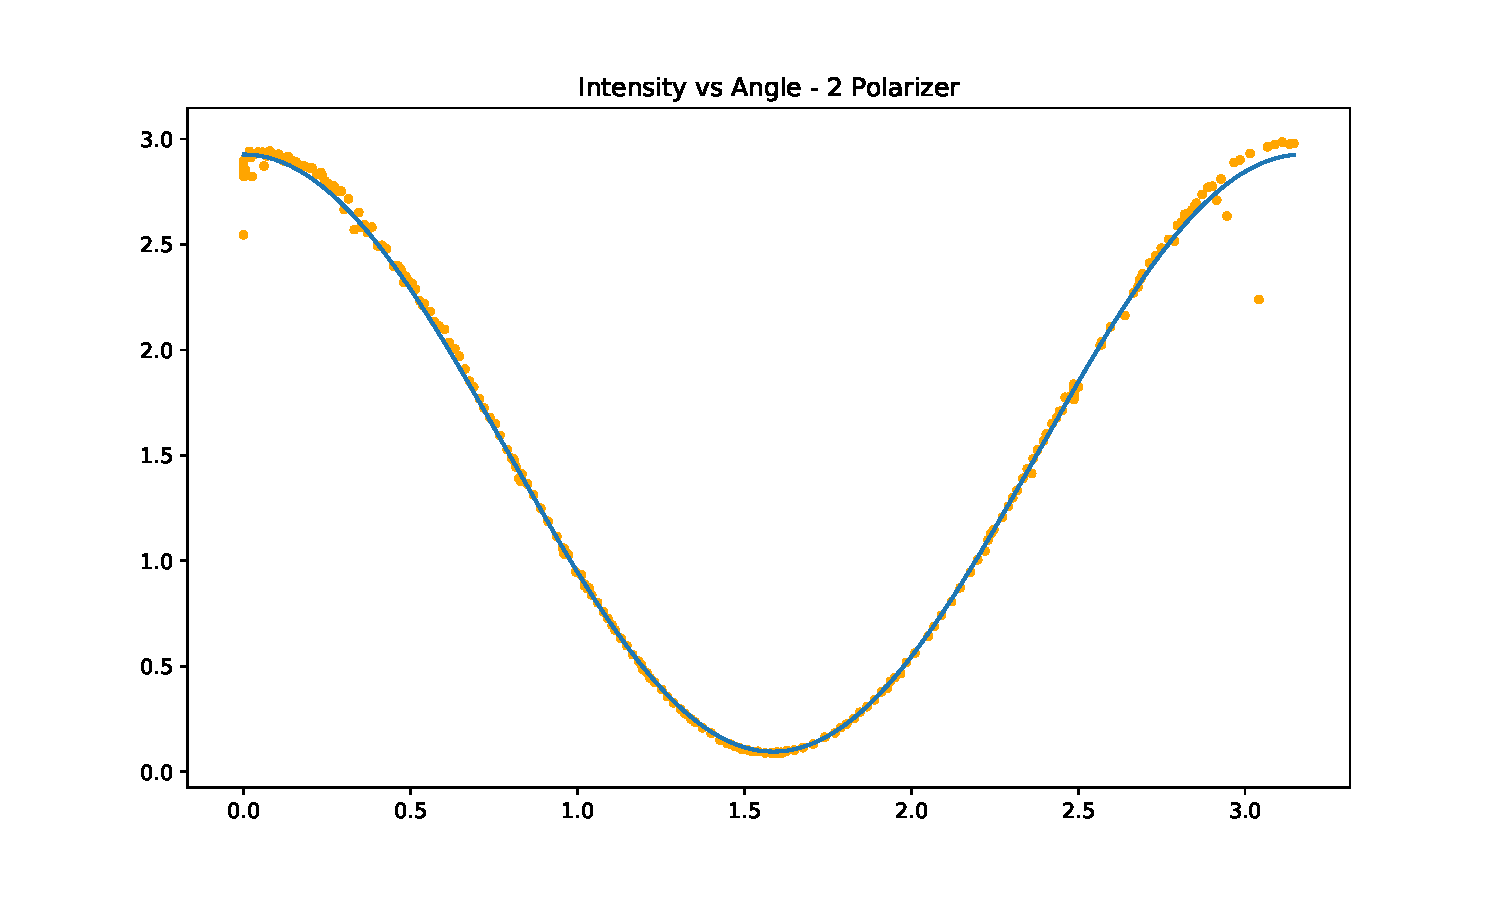
\includegraphics[width=\textwidth]{2pol-IntvsAng.pdf}	
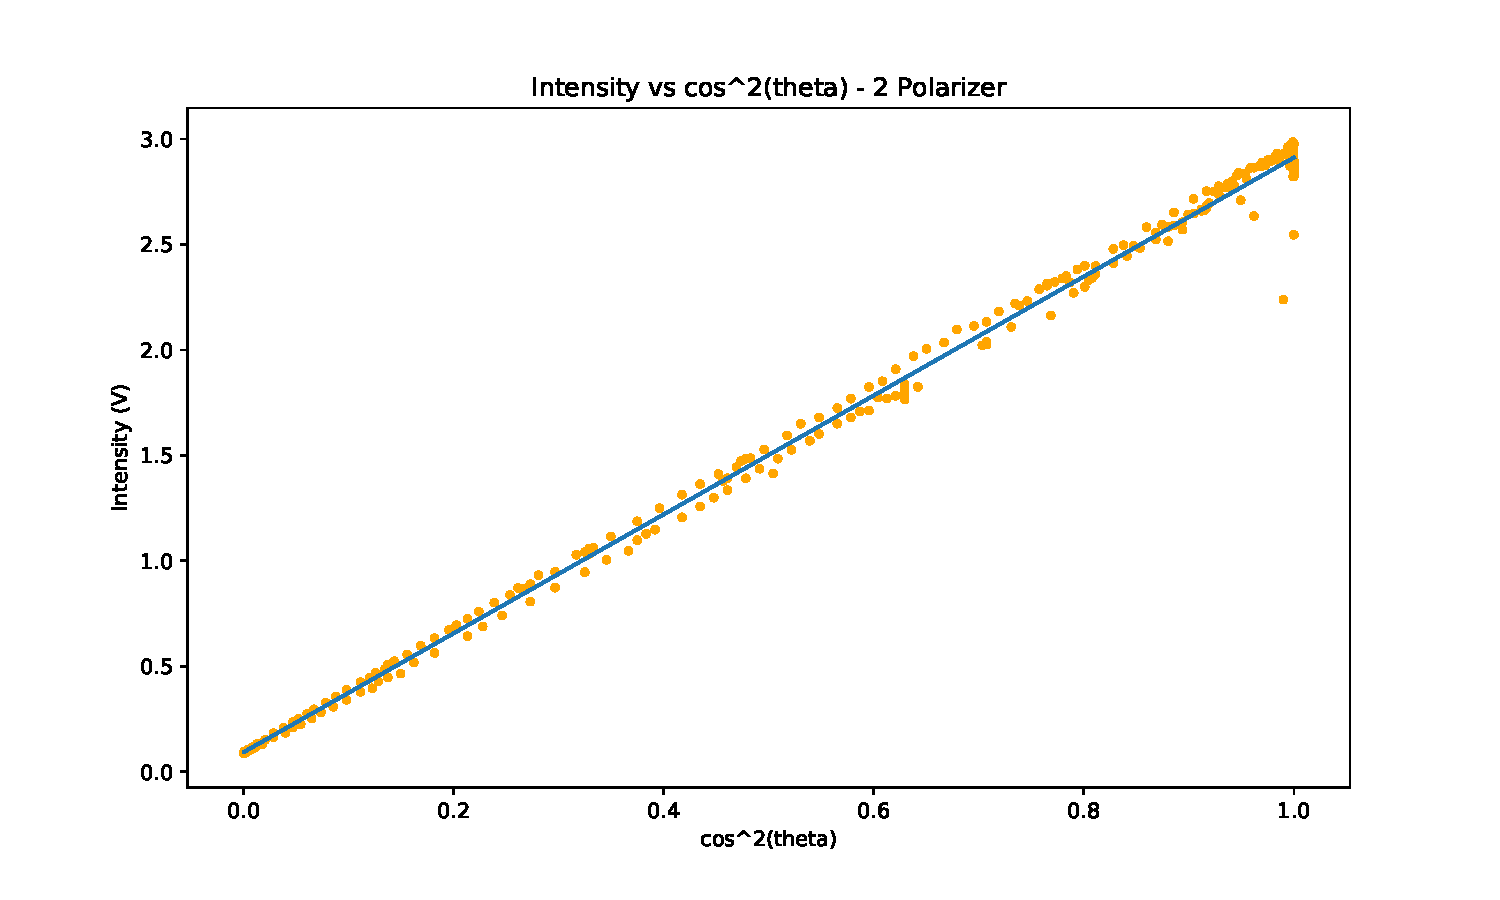
\includegraphics[width=\textwidth]{2pol-linear.pdf}
In the plot of Intensity vs $\cos^{2}\theta$ for the Malus' 2 polarizers exercise, we obtained a linear equation of:
\begin{center}
$I(\theta) = 2.820\cos^2\theta + 0.092$
\end{center}
This equation agrees with Malus' Law, since there is a small intercept value which can be attributed to error.

\subsubsection*{Malus' Law 3 Polarizers}
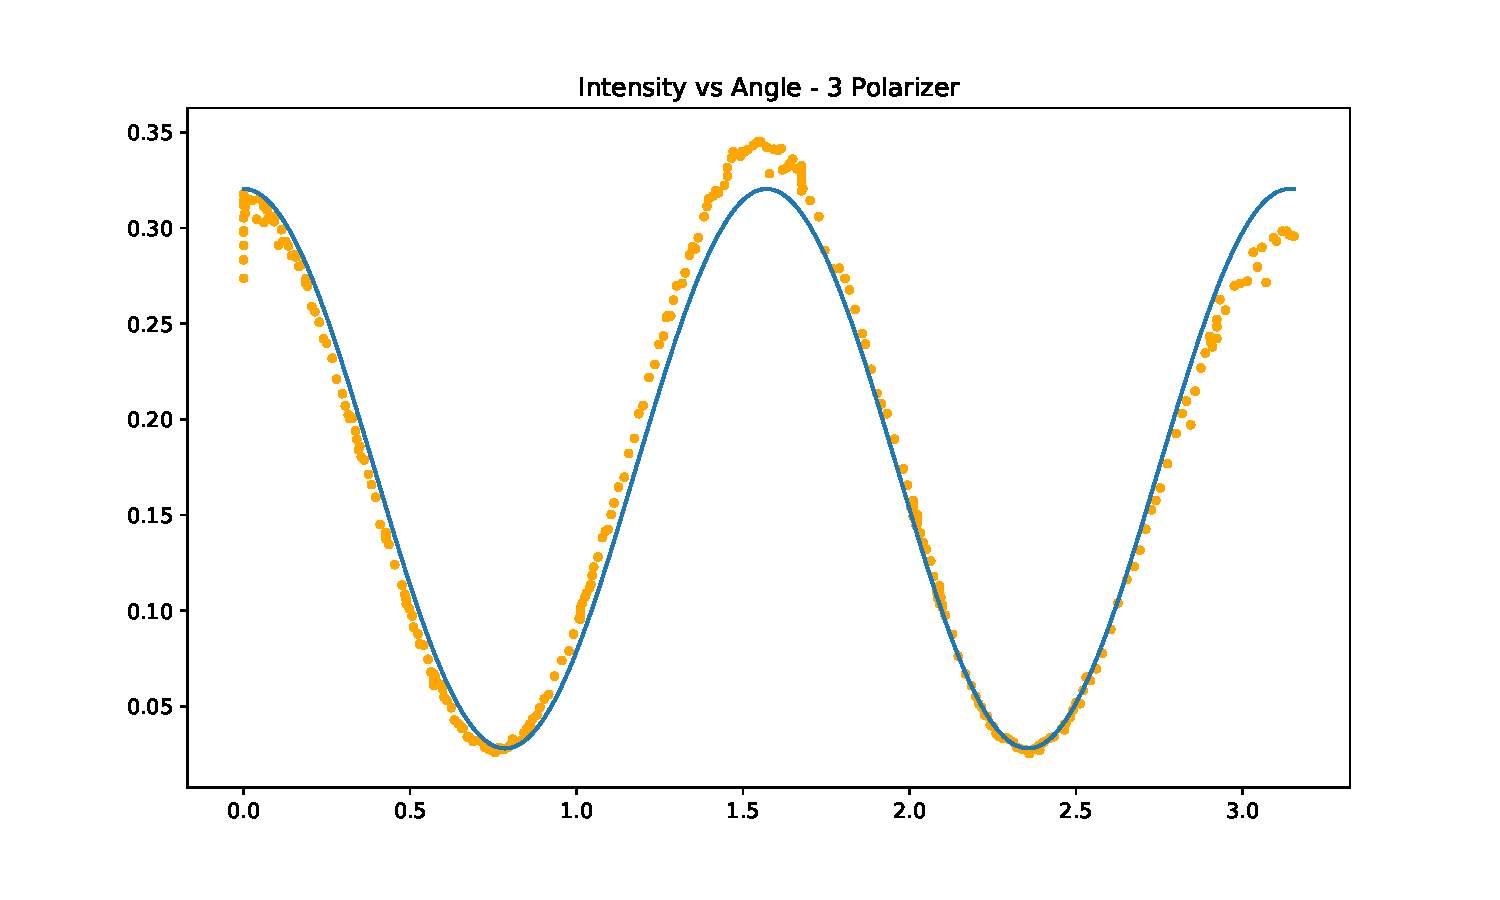
\includegraphics[width=\textwidth]{3pol-IntvsAng.pdf}
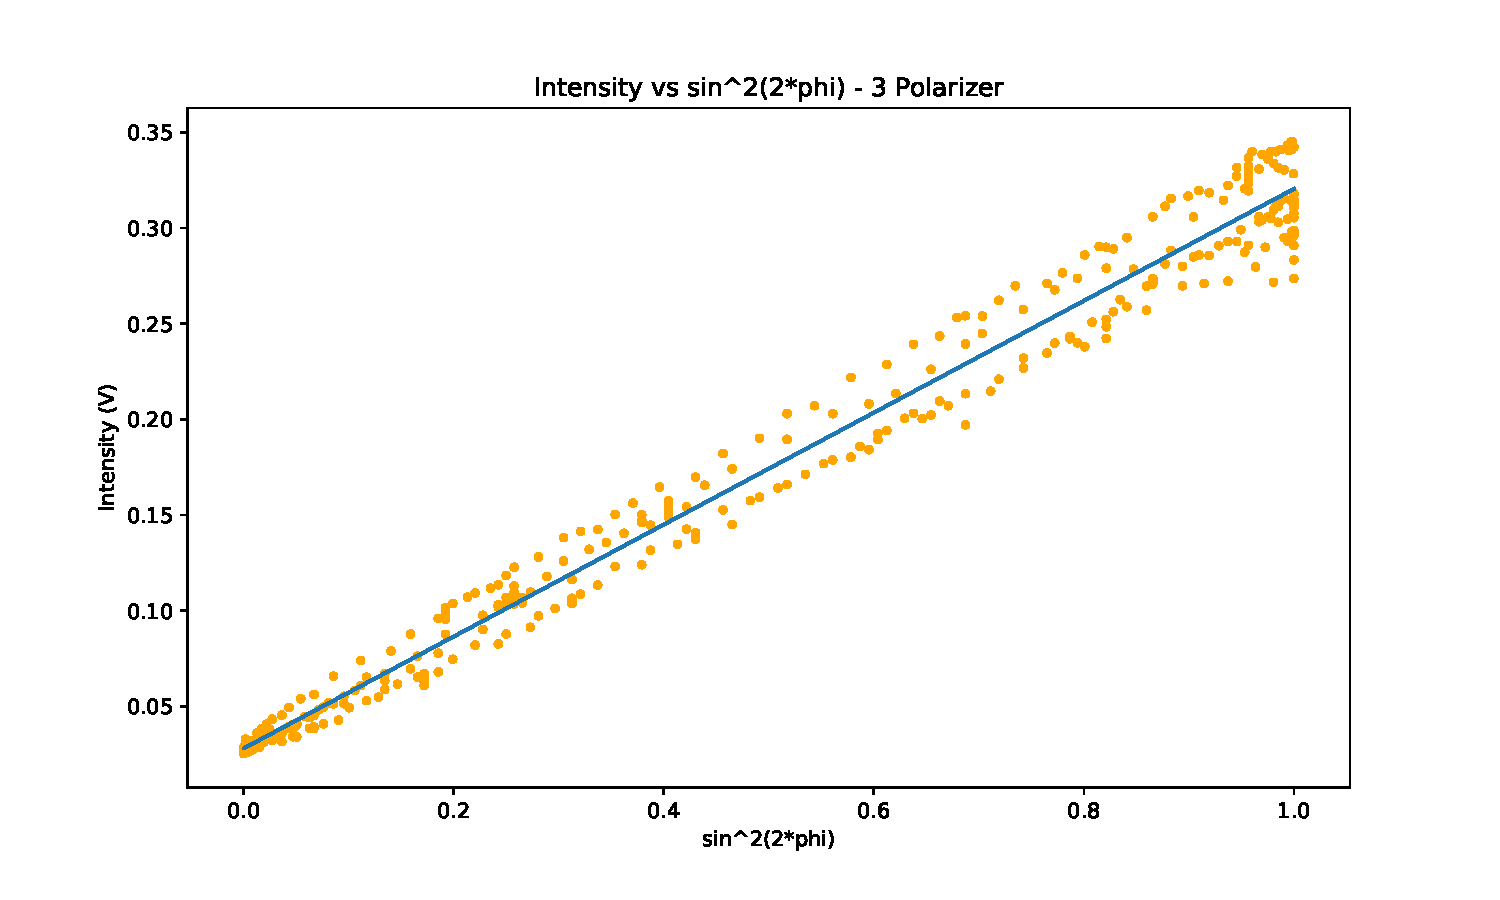
\includegraphics[width=\textwidth]{3pol-linear.pdf}
In the plot of Intensity vs $\sin^{2}(2\phi)$ for the Malus' 3 polarizers exercise, we obtained a linear equation of:
\begin{center}
$I_3 = 0.292\sin^{2}2\phi + 0.028$
\end{center} 

Two things that are different for the Intensity vs Angle graph for 3 polarizers compared to 2 polarizers is:
\begin{enumerate}
\item The 3 polarizers graph has two cycles, while the 2 polarizers graph only has one cycle.
\item The intensity values of the 3 polarizers is much smaller than the intensity values in the 2 polarizers.
\end{enumerate}

\subsubsection*{Brewster's Angle}
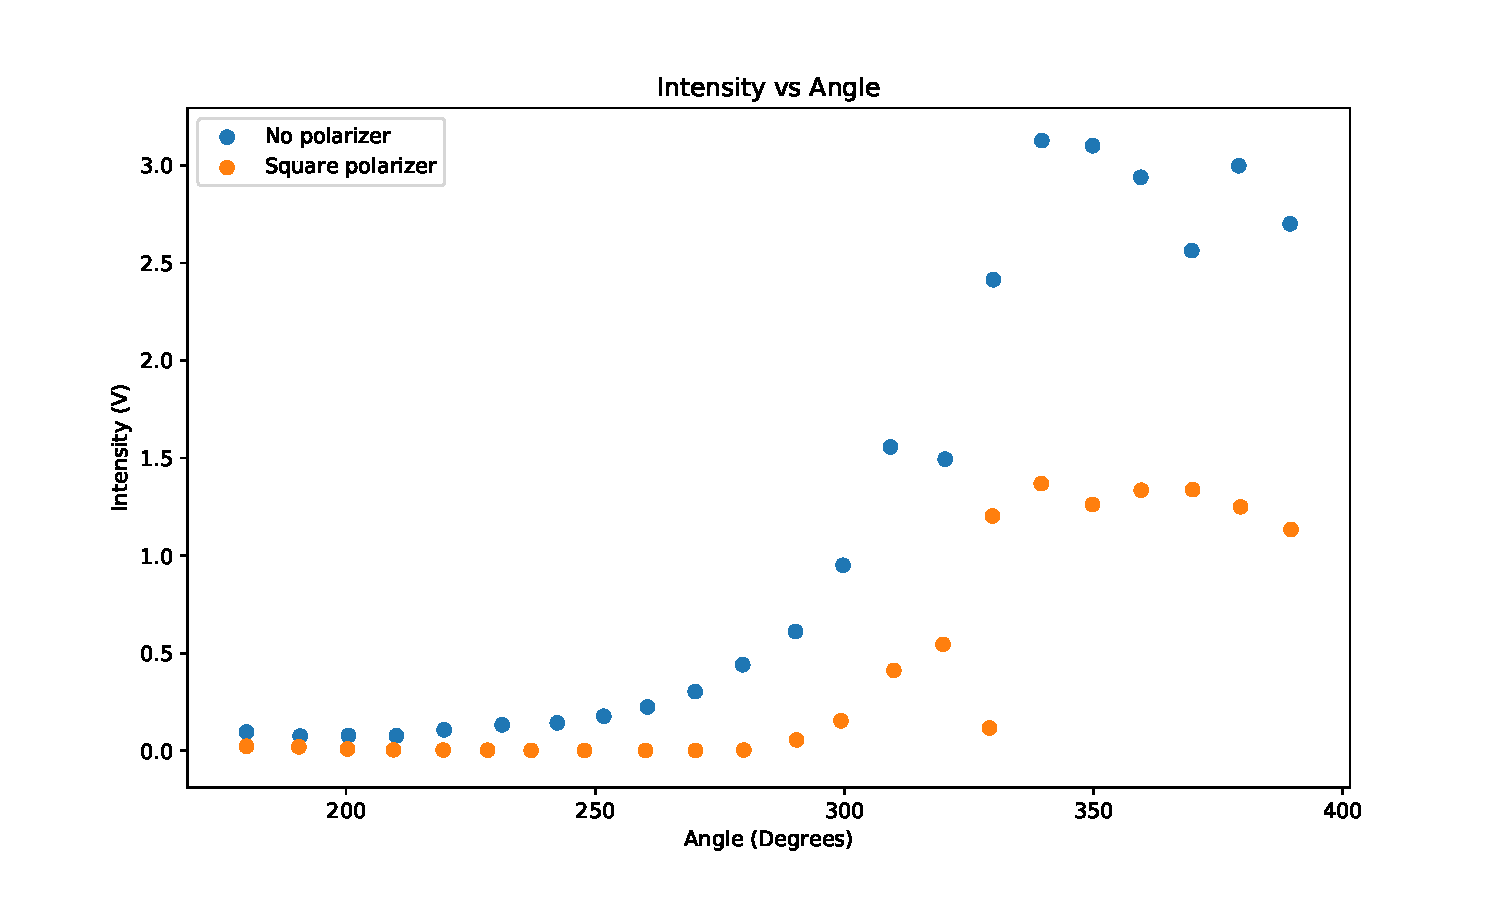
\includegraphics[width=\textwidth]{brewster-plot.pdf}
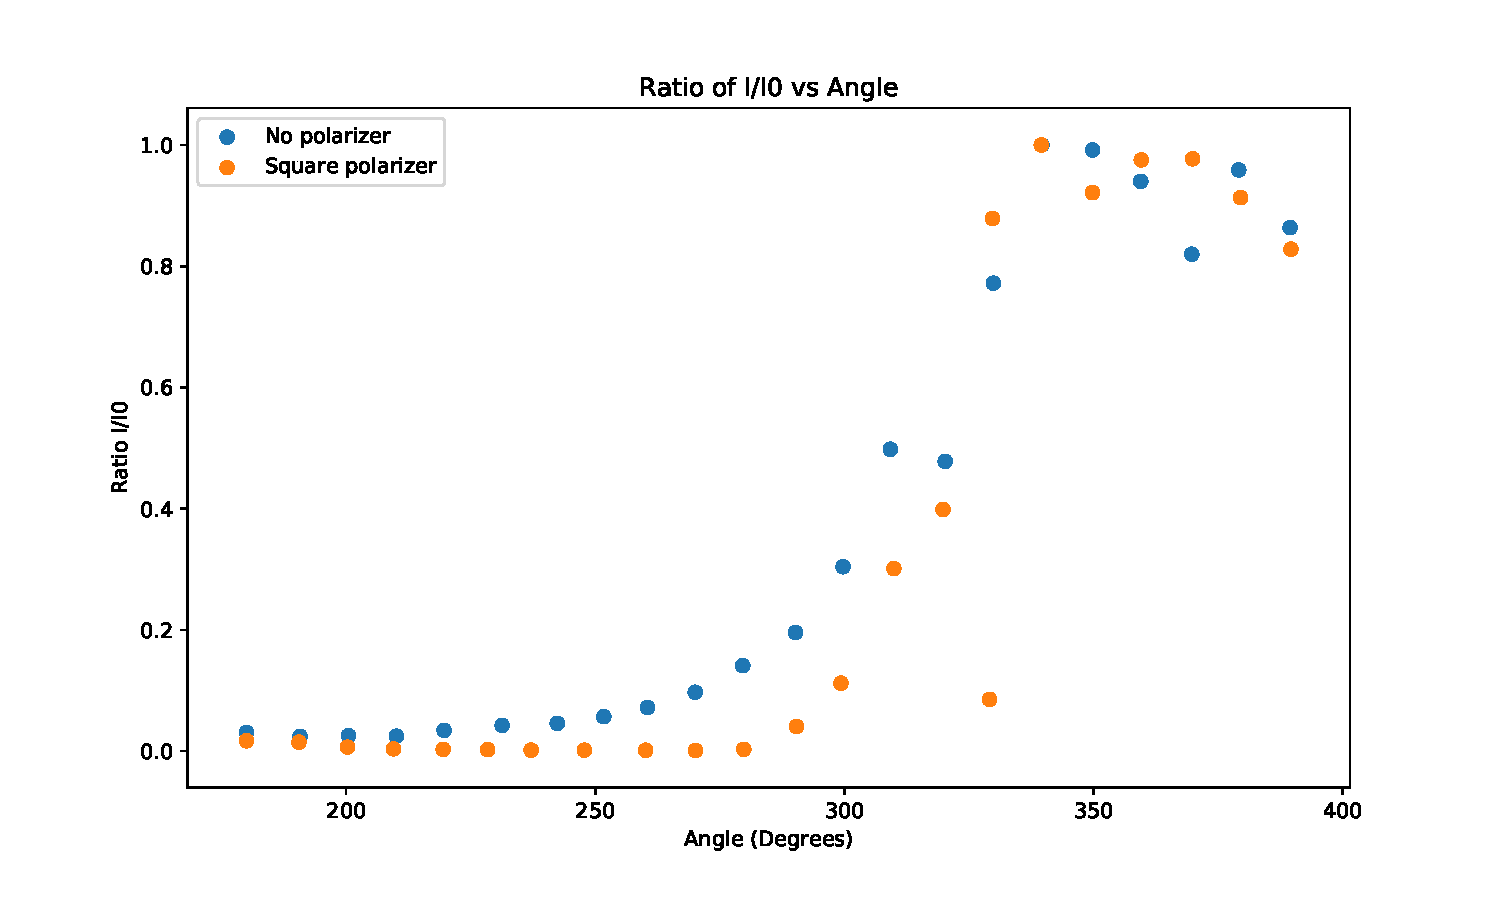
\includegraphics[width=\textwidth]{brewster-ratio.pdf}

In the two plots, the graph goes from 180 to 390 degrees. We started at 150 degrees and rotated until 360 degrees. Everything needs to be shifted to the left by 30 degrees so we later add 30 degrees in our calculations. Note that there are gaps in the plot because there were many data points with an intensity of less than 0 that were removed.

We can see from the second plot that the minimum of the square polarizer data occurs at about 260 degrees. Due to the translation issue, we add 30 to get 290 degrees. We call this angle $\alpha$, and we derived the following formula $\theta_p = \frac{\alpha}{2} - 90$. Dividing this angle by 2 gives 150 degrees. This is the angle to the normal, so we subtract 90 and obtain a final angle of 55 degrees.

Summarizing in a formula, we have: $\theta_p = \frac{\alpha}{2} - 90 =\frac{290}{2} - 90 = 55^{\circ}$ \\
\\
To obtain the index of refraction of acrylic, we use the equation:
\begin{center}
$n_2 = n_1\tan\theta_p = \tan(55^{\circ}) = 1.43$
\end{center}

Since $n_1 = 1$. \\
The actual index of refraction of acrylic is 1.49, so we have an error of about 4\%. \\
\\
Now we calculate the perpendicular reflectance and parallel reflectance using Fresnel's equations:
\begin{center}
$r_{\perp}=\frac{n_1\cos\theta_1-n_2\cos\theta_2}{n_1\cos\theta_1+n_2\cos\theta_2} = -0.342$
\\
$r_{\parallel}=\frac{n_1\cos\theta_2-n_2\cos\theta_1}{n_1\cos\theta_2+n_2\cos\theta_1} = 6.78\cdot10^{-17} \approx 0$
\end{center}
Where $\theta_2 = \sin^{-1}(\frac{n_1}{n_2}\sin\theta_1) \approx 35^{\circ}$ \\
\\
We can see above that the parallel reflectance is approximately 0. When this is true, we have the equation for Brewster's angle.

\section*{Malus' Law Questions}

\subsection*{Question 1}
For 3 polarizers, the angle between the middle polarizer and the first polarizer of $\phi = \frac{\pi}{4}$  achieves \textbf{maximum} transmission through all 3 polarizers. \\
\\
This is because $I_3 = I_2\cos^{2}(\frac{\pi}{2} - \phi_2) = I_1\cos^{2}\phi \cos^{2}(\frac{\pi}{2} - \phi) = \frac{I_1}{4}\sin^{2}(2\phi)$, so the angle of $\frac{\pi}{4}$ gives $I_3 = \frac{I_1}{4}\sin^{2}(2 \cdot \frac{\pi}{4}) = \frac{I_1}{4}$

\subsection*{Question 2}
To achieve \textbf{minimum} transmission through all 3 polarizers, the angle between the middle and first polarizers must be $\phi = 0$ or $\phi = \pi/2$. \\
\\
For $\phi = 0$: \ $I_3 = \frac{I_1}{4}\sin^{2}(2 \cdot 0) = 0$ \\
For $\phi = \pi/2$: \ $I_3 = \frac{I_1}{4}\sin^{2}(2 \cdot \frac{\pi}{2}) = 0$


\section*{Brewster's Angle Questions}

\subsection*{Question 1}
Brewster's angle would be less for light in air reflecting off of water, compared to light in air reflecting off of acrylic. This is because the index of refraction of water is smaller than the index of refraction of acrylic. This can be shown with a quick calculation:
\begin{center}
$\theta_p = \tan^{-1}(1.333) \approx 53^{\circ}$
\end{center}
This angle is smaller than the Brewster's angle for acrylic.

\subsection*{Question 2}
If we used a vertical polarizer, the data would look like data collected without a horizontal polarizer. This is because the light is very close to vertically polarized, so the polarizer does not affect the light passing through it.

\subsection*{Question 3}
Polarized sunglasses will polarize light passing through it, which reduces the intensity of the light. The axis of polarization is vertical. In order to check this, we would need to pass light through a rotary polarizer, and using the polarized sunglasses as an analyzer, we can measure the intensity of the light when it is vertically polarized.

\section*{Conclusion}
Our equations for the intensity output given by 2 polarizers and 3 polarizers agrees with Malus' Law. There were intercept terms but these can be attributed to error. We obtained a Brewster's angle of 55 degrees, and used this to derive the index of refraction for acrylic, where we got a value of 1.43, which has about 4\% error. There were multiple sources of error, including measurement error which is due to non-constant rotation of the lens and the disk during the trials. External sources of light from the computer and nearby lamps can affect the intensity of the light. There was also systematic error from our values for Brewster's angle; these values were not properly given in the correct units so we had to translate the angles to appropriate values.


\end{document}
